\documentclass[11pt, a4paper]{article}
\usepackage[english]{babel}
\usepackage{ragged2e}
\usepackage[utf8x]{inputenc}
\usepackage{amsmath}
\usepackage{float}
\usepackage{graphicx}
\usepackage[font=small,labelfont=bf]{caption}
\usepackage[top=2.0in, bottom=1.25in, left=1.20in, right=1.20in]{geometry}
\graphicspath{ {./Images/} }

\title{\vspace{-7cm}}
\author{}
\date{}

\begin{document}
\maketitle

\section{Literature Review / Background}

\subsection{Introduction}
This project is an attempt to combine multiple facets of game theory and artificial intelligence, in hope that the end result will be educational and/or useful to the fields. There are multiple stepping stones within the fields of game theory, mathematics, etc. which need to be examined in order to gain a further understanding of the project, which we will look at in this section.

\subsection{Brief History of Game Theory}
Game theory is the study of behaviours and mathematical models which result from the decisions and strategies of two or more economically rational players in either cooperative or non-cooperative strategy games. Applications of game theory have manifested in social science, psychology, mathematics and many more fields of study; however, the root interactions lie in strategic games such as the prisoner's dilemma or tit-for-tat. Game theory was introduced and popularised by mathematician John von Neumann, who first proved an optimal strategy for zero-sum games with perfect information such as chess or go called the minimax theorem in 1928. This theorem indicates that in such games, there is a pair of strategies for each player which allows them to minimise their maximum losses, while considering all responsive moves of the opponent. \\
\noindent
After von Neumann published his initial paper on game theory, he published a book co-authored by economist Oskar Morgenstein entitled, "Theory of Games and Economic Behaviour". Within this book, von Neumann fixates mainly on non-cooperative games and/or zero-sum games; but most importantly, identified a method of finding consistent solutions and strategies for both players in two-person zero-sum games. This work became a milestone for game theory as it established a foundation for becoming a unique discipline. \\
\noindent
Following this, numerous advancements in game theory occurred during the 1950s - mathematicians Merrill Flood and Melvin Dresher experimented mathematical and game versions of the prisoner's dilemma for the American think tank corporation, RAND (Research and Development). In the same year, John Forbes Nash Jr published his dissertation on non-cooperative games which contained the first definitions of the Nash equilibrium - an important milestone for adaptive strategy in game theory. He proved that in every n-player non-zero sum game, a Nash equilibrium existed, assuming the game had a finite number of actions. This was a continuation of the work from von Neumann and Morgenstein in their 1944 book, which only covered two person zero-sum games, and was restrained by the implications of 'rational' behaviour. \\
\noindent
In 1980, political scientist Robert Axelrod set up a multi-agent tournament for the iterated/repeated prisoner's dilemma. Multiple well-known game theorists from different professions such as psychology, political science, economics, mathematics and more submitted 14 FORTRAN (Formula Translation) programs for the agents to follow as implicit strategies. In this tournament, agents would play against each other for 200 rounds - mutual cooperation would yield 3 points, mutual defection 1 point, single defection 5 points and single cooperation 0 points. The winning strategy was a simple tit-for-tat program which cooperated on the first turn, then repeated the opponents previous move for each subsequent turn. This strategy ended the tournament with an average of 504.5 points of a maximum 1000. \\

\subsection{Prisoner's Dilemma}
The prisoner's dilemma is one of the fundamental games of game theory which shows the payoffs and consequences of two 'players' acting in their own self interests. This summary, cited from britannica.com, is a model version of the prisoner's dilemma: \\

\noindent
"\textit{Two prisoners are accused of a crime. If one confesses and the other does not, the one who confesses will be released immediately and the other will spend 20 years in prison. If neither confesses, each will be held only a few months. If both confess, they will each be jailed 15 years. They cannot communicate with one another. Given that neither prisoner knows whether the other has confessed, it is in the self-interest of each to confess himself. Paradoxically, when each prisoner pursues his self-interest, both end up worse off than they would have been had they acted otherwise.}" \\

\noindent
The first examples of the prisoner's dilemma being used in the context of game theory date back to the 1950s, by Merrill Flood and Melvin Dresher who devised puzzles and experiments using the structure of the dilemma - mainly an attempt to verify the usefulness of a non-cooperative Nash equilibrium. In this experiment, Flood and Dresher ran 100 games between two human players - in which player 1 (economist Armen Alchian) cooperated 68 times, while player 2 (mathematician John Williams) cooperated 78 times. In game theory, if a strategic game exists with the possibility for a various number of possible outcomes, a payoff matrix can be used to visually represent the benefits and consequences of each outcome. For the prisoner's dilemma, a typical payoff matrix would look as such:

\begin{figure}[h]
	\centering
		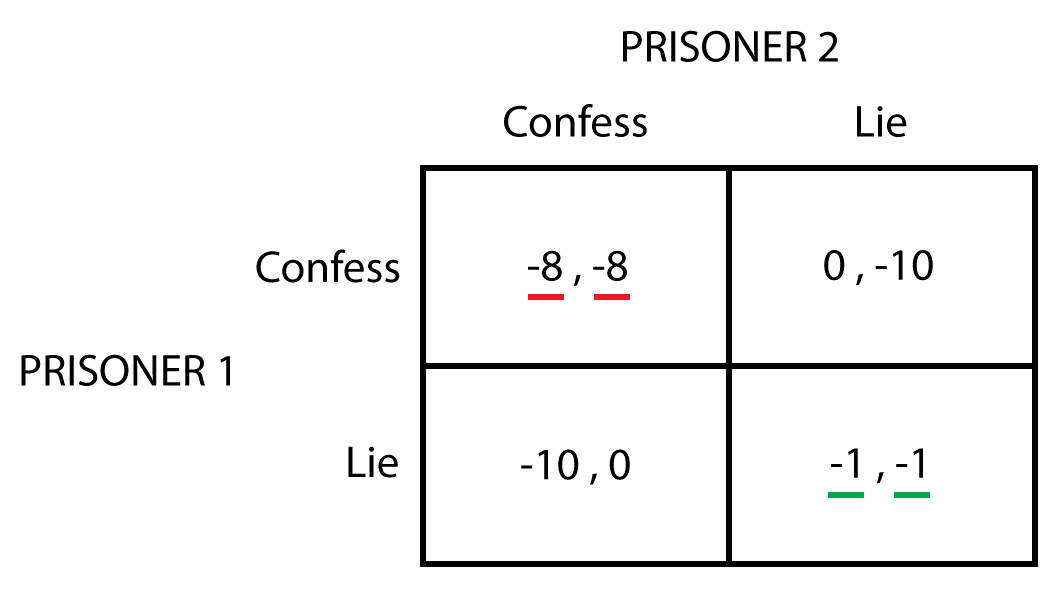
\includegraphics[width=0.6\textwidth]{DilemmaPayoffMatrix}
		\caption{Prisoner's Dilemma Payoff Matrix}
\end{figure}

\noindent
As you can see, the prisoner's would achieve the best possible equal payoff if they consistently chose to confess, but a prisoner could achieve a higher payoff if they were to follow their own self interests. However, the payoff matrix in this experiment looked like this:

\begin{figure}[H]
	\centering
		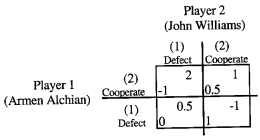
\includegraphics[width=0.5\textwidth]{FloodDresherPayoff}
		\caption{Flood-Dresher Experiment Payoff Matrix}
\end{figure}

\noindent
In the Flood-Dresher experiment, the restraints can be thought of as 'unfair' as human players have a level of empathy and other emotion which may sway their decision for reasons an A.I. program would never follow. Such an example would be the comments which player 1 made in their log of comments. Alchian, or player 1, wrote comments such as "He does not want to trick me. He is satisfied. I must teach him to share", while player 2 Williams wrote comments such as "A shiftless individual - opportunist, knave" (de Herdt, 2003, p. 189) just a turn apart from each other. Many economists, game theorists and mathematicians believe that the results of this experiment may have been swayed slightly due to each player being empathetic or vindictive at numerous points in the game. % needs more content

\subsection{Nash Equilibrium}
In 1950, John Forbes Nash Jr. published his dissertation entitled, "Non-cooperative Games". Within this dissertation was proof which indicated that within a two person zero-sum game, there exists an 'equilibrium point' for both players. This equilibrium was described in the paper as such, "Thus an equilibrium point is an n-tuple such that each player's mixed strategy maximizes his pay-off if the strategies of the others are held fixed. Thus each player's strategy is optimal against those of the others" (Nash, 1950, p. 3). Simply put, Nash was illustrating that within a two person game in which one player's benefit is a direct loss for the opponent, there lies a state in which neither player has any incentive to switch strategies, as it will not benefit their payoff - thus, the game sits at an equilibrium. The simplest, and most likely quickest way to prove the existence of a Nash equilibrium would be as follows:

\begin{figure}[H]
	\centering
		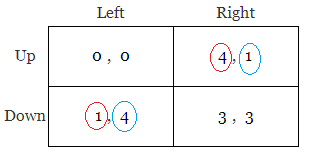
\includegraphics[width=0.5\textwidth]{ModelMatrix}
		\caption{Example Matrix}
\end{figure}

\noindent
Most proofs of equilibria exist if a certain number of conditions are met. Given a model payoff matrix, figure 3, our conditions for a pure/mixed strategy Nash equilibrium are as follows:

\begin{itemize}
  \item The first player's best response is the same against any potential move of the opponent (red circle).
  \item The second player's best response is the same against any potential move of the opponent (blue circle).
  \item Nash equilibrium = (Up, Right),(Down, Left).
\end{itemize}

\noindent
There are a few ways of proving the existence of a Nash equilibrium within games in a more detailed way - within Nash's dissertation, he chose to speak about the 'generalised' Kakutani fixed point theorem, and the Brouwer fixed point theorem.

\subsubsection{Kakutani's Fixed Point Theorem}
The Kakutani fixed point theorem states that a common fixed point exists within a collection of maps defined on non-empty, convex and compact subsets. Given the following scenario from San Jose State University: \\

\noindent
"\textit{Let M be a compact, convex subset of Euclidean n-space. \footnote{A Euclidean space is sometimes known as n-space, and is simply the space of all n-tuples of real numbers.} Let T be a continuous set-valued function on M; i.e., a mapping from M to the set of all subsets of M, T→P(M). If T is such that T(x) is convex for all x belonging to M then there exists a z such that T(z) contains z."} \\

\noindent
This theorem can be proven if the following conditions are satisfied:

\begin{itemize}
  \item M is a non-empty, convex and compact set.
  \item T(x) is non-empty for all x ∈ M.
  \item For all x ∈ M, T(x) is a convex set.
  \item T(x) has a closed graph, i.e. if \{x\textsuperscript{n}, y\textsuperscript{n}\} → \{x, y\} with y\textsuperscript{n} ∈ T(x\textsuperscript{n}), then y ∈ T(x).
\end{itemize}

\noindent
If satisfied, a fixed point exists within T.

\clearpage

\end{document}